% Gabarit pandoc des corrigés publiés (brut et guidé). Contenu sans marque ni nom de site.
% Compilation : lualatex (latexmk -lualatex).
% Le Markdown reste la source unique : ne pas éditer ce fichier .tex à la main.
\documentclass[11pt,a4paper]{article}

% --- Moteur, polices (Latin Modern) et langue ---------------------------------
\usepackage{iftex}
\ifLuaTeX\else\errmessage{Ce document se compile avec lualatex}\fi
\usepackage{amsmath,amssymb,mathtools}
\usepackage{fontspec}
% mathrm=sym : \mathrm prend ses glyphes dans la police mathématique (ℓ, μ, Ω), comme KaTeX.
\usepackage[math-style=TeX,bold-style=TeX,mathrm=sym]{unicode-math}
% Repli pour les glyphes absents de Latin Modern (indices et exposants Unicode,
% flèches, filets des schémas en texte, symboles) : DejaVu, puis Latin Modern Math
% (ℓ, lettres mathématiques Unicode des légendes).
\directlua{
  luaotfload.add_fallback("repliTexte", {"DejaVuSerif:mode=harf;", "DejaVuSans:mode=harf;", "file:latinmodern-math.otf:mode=harf;"})
  luaotfload.add_fallback("repliMono", {"DejaVuSansMono:mode=harf;", "DejaVuSans:mode=harf;", "file:latinmodern-math.otf:mode=harf;"})
}
\setmainfont{Latin Modern Roman}[RawFeature={fallback=repliTexte}]
\setsansfont{Latin Modern Sans}[RawFeature={fallback=repliTexte}]
\setmonofont{Latin Modern Mono}[RawFeature={fallback=repliMono}]
\setmathfont{Latin Modern Math}
\usepackage[french]{babel}
\frenchsetup{SmallCapsFigTabCaptions=false}

% --- Mise en page --------------------------------------------------------------
\usepackage[a4paper,margin=2.2cm,headheight=14pt,footskip=1.2cm]{geometry}
\usepackage{microtype}
\setlength{\emergencystretch}{4em}
\tolerance=1500
\setlength{\parindent}{0pt}
\setlength{\parskip}{0.55\baselineskip plus 2pt minus 1pt}
\usepackage{xcolor}
% Gris nommés : babel-french rend « ! » actif dans le document.
\definecolor{gris2}{gray}{0.98}
\definecolor{gris3}{gray}{0.97}
\definecolor{gris5}{gray}{0.95}
\definecolor{gris35}{gray}{0.65}
\definecolor{gris40}{gray}{0.60}
\definecolor{gris45}{gray}{0.55}
\definecolor{gris50}{gray}{0.50}
\definecolor{gris55}{gray}{0.45}
\definecolor{gris60}{gray}{0.40}
\definecolor{gris65}{gray}{0.35}
\definecolor{gris70}{gray}{0.30}
\definecolor{gris80}{gray}{0.20}
\definecolor{gris85}{gray}{0.15}
\usepackage{graphicx}
\usepackage{float}
\usepackage{caption}
\captionsetup{font=small,labelformat=empty,justification=centering}
\usepackage{booktabs,longtable,array,multirow,calc}
\usepackage{siunitx}
\sisetup{locale=FR}
\usepackage[version=4]{mhchem}
\usepackage{listings}
\usepackage{fancyhdr}
\usepackage{lastpage}
\usepackage[most]{tcolorbox}
\usepackage{enumitem}
\setlist{nosep,leftmargin=*,topsep=2pt}
\usepackage[hidelinks,unicode]{hyperref}
\usepackage{bookmark}
\hypersetup{pdftitle={G2E BCPST — Mathématiques 2026},pdfauthor={Rédigé par IA},pdfcreator={LaTeX},pdfsubject={Corrigé brut}}
\usepackage{xurl}

% --- Pandoc : listes, tableaux, figures ----------------------------------------
\providecommand{\passthrough}[1]{#1}
\providecommand{\tightlist}{\setlength{\itemsep}{0pt}\setlength{\parskip}{0pt}}

\makeatletter
\def\maxwidth{\ifdim\Gin@nat@width>\linewidth\linewidth\else\Gin@nat@width\fi}
\def\maxheight{\ifdim\Gin@nat@height>0.55\textheight 0.55\textheight\else\Gin@nat@height\fi}
\makeatother
\setkeys{Gin}{width=\maxwidth,height=\maxheight,keepaspectratio}
\setcounter{secnumdepth}{-\maxdimen}
\providecommand{\pandocbounded}[1]{#1}

% --- Code (listings) -----------------------------------------------------------
\lstset{
  basicstyle=\ttfamily\small,
  columns=fullflexible,
  keepspaces=true,
  breaklines=true,
  breakatwhitespace=false,
  postbreak=\mbox{\textcolor{gris50}{$\hookrightarrow$}\space},
  frame=single,
  rulecolor=\color{gris35},
  framesep=4pt,
  xleftmargin=5pt,xrightmargin=5pt,
  backgroundcolor=\color{gris3},
  keywordstyle=\bfseries,
  commentstyle=\color{gris65},
  stringstyle=\color{gris80},
  showstringspaces=false,
  tabsize=4,
  extendedchars=true,
  aboveskip=6pt,belowskip=6pt,
}

% --- Macros des corrigés (KaTeX ↔ LaTeX) ---------------------------------------
% Les corrigés sont écrits pour KaTeX : on définit ici ce que KaTeX connaît et
% que LaTeX n'a pas, sans jamais retoucher le Markdown.
\providecommand{\R}{\mathbb{R}}
\providecommand{\N}{\mathbb{N}}
\providecommand{\Z}{\mathbb{Z}}
\providecommand{\Q}{\mathbb{Q}}
\providecommand{\C}{\mathbb{C}}
\providecommand{\dd}{\mathrm{d}}
\providecommand{\llbracket}{\lBrack}
\providecommand{\rrbracket}{\rBrack}
\providecommand{\lBrace}{\lbrace}
\providecommand{\rBrace}{\rbrace}
\providecommand{\Box}{\square}
\providecommand{\Diamond}{\lozenge}
\providecommand{\varnothing}{\emptyset}
\providecommand{\argmax}{\operatorname*{arg\,max}}
\providecommand{\argmin}{\operatorname*{arg\,min}}
\renewcommand{\leq}{\leqslant}
\renewcommand{\geq}{\geqslant}

% Équation hors texte : réduite à la largeur de la ligne si elle déborde.
\newsavebox{\boiteequation}
\newcommand{\equationajustee}[1]{%
  \sbox{\boiteequation}{$\displaystyle #1$}%
  \ifdim\wd\boiteequation>\linewidth
    \[\resizebox{\linewidth}{!}{\usebox{\boiteequation}}\]%
  \else
    \[#1\]%
  \fi}

% --- Encadrés pédagogiques (sobres, lisibles en noir et blanc) -----------------
\tcbset{
  encadre/.style={
    enhanced,breakable,sharp corners,
    colback=white,colframe=gris55,
    boxrule=0.4pt,leftrule=2.2pt,
    left=6pt,right=6pt,top=3pt,bottom=3pt,
    before skip=6pt,after skip=6pt,
    fonttitle=\bfseries\small,coltitle=black,
    attach title to upper,after title={\quad},
    parbox=false,
  }
}
\newtcolorbox{indication}[1]{encadre,colframe=gris45,colback=gris2,title={Indication~#1}}
\newtcolorbox{methode}{encadre,colframe=gris70,title={Méthode}}
\newtcolorbox{piege}{encadre,colframe=gris85,boxrule=0.8pt,leftrule=2.2pt,title={Piège}}
\newtcolorbox{jury}{encadre,colframe=gris60,colback=gris5,title={Jury}}
\newtcolorbox{encadrenote}{encadre,colframe=gris40}

% --- Titres de section ---------------------------------------------------------
\usepackage{titlesec}
\titleformat{\section}{\Large\bfseries}{}{0pt}{}
\titleformat{\subsection}{\large\bfseries}{}{0pt}{}
\titleformat{\subsubsection}{\normalsize\bfseries}{}{0pt}{}
\titlespacing*{\section}{0pt}{14pt plus 4pt minus 2pt}{6pt}
\titlespacing*{\subsection}{0pt}{10pt plus 3pt minus 2pt}{4pt}
\titlespacing*{\subsubsection}{0pt}{8pt plus 2pt minus 2pt}{2pt}

% --- En-tête et pied de page ---------------------------------------------------
\pagestyle{fancy}
\fancyhf{}
\fancyhead[L]{\small\textsc{Corrigé brut} · G2E BCPST}
\fancyhead[R]{\small Maths 2026}
\fancyfoot[L]{\footnotesize Corrigé rédigé par IA, non officiel}
\fancyfoot[R]{\footnotesize \thepage\,/\,\pageref*{LastPage}}
\renewcommand{\headrulewidth}{0.4pt}
\renewcommand{\footrulewidth}{0pt}
\fancypagestyle{plain}{\fancyhf{}\fancyfoot[R]{\footnotesize \thepage\,/\,\pageref*{LastPage}}\fancyfoot[L]{\footnotesize Corrigé rédigé par IA, non officiel}\renewcommand{\headrulewidth}{0pt}}

\begin{document}
\thispagestyle{plain}
\begin{center}
  {\small\scshape Corrigé brut}\par\smallskip
  {\LARGE\bfseries G2E BCPST — Mathématiques 2026\par}\medskip
  {\large G2E · BCPST · Maths · 2026\par}
\end{center}
\vspace{2pt}\hrule\vspace{8pt}

\emph{Corrigé rédigé par IA, non officiel. Signalez toute erreur.}

Épreuve de 4 heures, calculatrices programmables et alphanumériques interdites, aucun document. Deux problèmes indépendants.

\hypertarget{probluxe8me-1}{%
\section{Problème 1}\label{probluxe8me-1}}

Dans tout le problème, le repère du plan est orthonormal.

\hypertarget{partie-a-calcul-dune-intuxe9grale-uxe0-laide-de-deux-fonctions-intermuxe9diaires}{%
\subsection{Partie A : Calcul d'une intégrale à l'aide de deux fonctions intermédiaires}\label{partie-a-calcul-dune-intuxe9grale-uxe0-laide-de-deux-fonctions-intermuxe9diaires}}

Sur \([1,+\infty[\) : \(\varphi(t)=\dfrac{t^2-1}{t^2+1}\) et \(\psi(t)=\dfrac{t}{t^2+1}+\arctan(t)\).

\hypertarget{a}{%
\subsubsection{1. (a)}\label{a}}

Les fonctions \(t\mapsto t^2-1\), \(t\mapsto t\) et \(t\mapsto t^2+1\) sont polynomiales, donc de classe \(\mathcal C^1\) sur \(\mathbb R\).

De plus, \(t^2+1\geqslant 1>0\) ne s'annule pas. Par quotient, \(\varphi\) et \(t\mapsto t/(t^2+1)\) sont de classe \(\mathcal C^1\) sur \([1,+\infty[\).

La fonction \(\arctan\) est de classe \(\mathcal C^1\) sur \(\mathbb R\), de dérivée \(t\mapsto 1/(1+t^2)\).

Par somme, \(\psi\) est de classe \(\mathcal C^1\) sur \([1,+\infty[\).

\equationajustee{\varphi'(t)=\frac{2t(t^2+1)-(t^2-1)\,2t}{(t^2+1)^2}=\frac{4t}{(t^2+1)^2}.}

\equationajustee{\begin{aligned}
\psi'(t)&=\frac{(t^2+1)-2t^2}{(t^2+1)^2}+\frac{1}{t^2+1}\\
&=\frac{1-t^2+t^2+1}{(t^2+1)^2}\\
&=\frac{2}{(t^2+1)^2}.
\end{aligned}}

Ainsi, pour tout \(t\geqslant 1\) :

\equationajustee{\boxed{\begin{aligned}
\varphi'(t)&=\frac{4t}{(t^2+1)^2}\\
\psi'(t)&=\frac{2}{(t^2+1)^2}
\end{aligned}}}

\hypertarget{b}{%
\subsubsection{1. (b)}\label{b}}

Pour \(t\geqslant 1\), on a \(4t>0\), donc \(\varphi'(t)>0\).

\textbf{\(\varphi\) est strictement croissante sur \([1,+\infty[\).}

\(\varphi\) est continue en \(1\), donc

\equationajustee{\begin{aligned}
\lim_{t\to1}\varphi(t)&=\varphi(1)\\
&=\frac{0}{2}\\
&=0.
\end{aligned}}

En \(+\infty\), pour \(t\neq 0\) :

\equationajustee{\varphi(t)=\frac{1-1/t^2}{1+1/t^2}\longrightarrow 1.}

\equationajustee{\boxed{\begin{aligned}
\lim_{t\to 1}\varphi(t)&=0\\
\lim_{t\to+\infty}\varphi(t)&=1
\end{aligned}}}

Continue et strictement croissante, \(\varphi\) réalise donc une bijection de \([1,+\infty[\) sur \([0,1[\).

\hypertarget{a-1}{%
\subsubsection{2. (a)}\label{a-1}}

\(f:x\mapsto\sqrt{1-x^2}\) est continue sur \([-1,1]\), donc \(I=\int_0^1 f(x)\,\mathrm dx\) est l'intégrale d'une fonction continue sur un segment.

\emph{Hypothèses.} Soit \(A\geqslant 1\). Sur le segment \([1,A]\), \(\varphi\) est de classe \(\mathcal C^1\) (question 1(a)).

Elle est à valeurs dans \([0,\varphi(A)]\subset[0,1]\) (question 1(b)), intervalle sur lequel \(f\) est continue.

Le théorème de changement de variable donne, avec \(x=\varphi(t)\) et \(\mathrm dx=\varphi'(t)\,\mathrm dt\) :

\equationajustee{\int_{0}^{\varphi(A)}f(x)\,\mathrm dx=\int_1^A f(\varphi(t))\,\varphi'(t)\,\mathrm dt .}

\emph{Calcul.} On a

\equationajustee{\begin{aligned}
1-\varphi(t)^2&=\frac{(t^2+1)^2-(t^2-1)^2}{(t^2+1)^2}\\
&=\frac{4t^2}{(t^2+1)^2}.
\end{aligned}}

Comme \(t>0\), on en déduit \(f(\varphi(t))=\dfrac{2t}{t^2+1}\). D'où

\equationajustee{f(\varphi(t))\,\varphi'(t)=\frac{2t}{t^2+1}\cdot\frac{4t}{(t^2+1)^2}=\frac{8t^2}{(t^2+1)^3}.}

\emph{Passage à la limite.} \(F:y\mapsto\int_0^y f\) est continue sur \([0,1]\) (primitive de \(f\) continue).

De plus, \(\varphi(A)\to 1\) quand \(A\to+\infty\), donc

\equationajustee{\int_0^{\varphi(A)}f=F(\varphi(A))\xrightarrow[A\to+\infty]{}F(1)=I.}

Ainsi \(\int_1^A\frac{8t^2}{(t^2+1)^3}\,\mathrm dt\) admet la limite finie \(I\) : l'intégrale impropre converge et

\equationajustee{\boxed{I=\int_1^{+\infty}\frac{8t^2}{(t^2+1)^3}\,\mathrm dt.}}

\hypertarget{b-1}{%
\subsubsection{2. (b)}\label{b-1}}

Soit \(A\geqslant1\). On pose, sur \([1,A]\), les fonctions de classe \(\mathcal C^1\) suivantes :

\equationajustee{\begin{aligned}
u(t)&=t, & u'(t)&=1,\\
v(t)&=-\frac{2}{(t^2+1)^2}, & v'(t)&=\frac{8t}{(t^2+1)^3}.
\end{aligned}}

On a donc \(u(t)v'(t)=\dfrac{8t^2}{(t^2+1)^3}\). Par intégration par parties :

\equationajustee{\begin{aligned}
\int_1^A\frac{8t^2}{(t^2+1)^3}\,\mathrm dt&=\Big[-\frac{2t}{(t^2+1)^2}\Big]_1^A+\int_1^A\frac{2\,\mathrm dt}{(t^2+1)^2}\\
&=-\frac{2A}{(A^2+1)^2}+\frac12+2\int_1^A\frac{\mathrm dt}{(t^2+1)^2}.
\end{aligned}}

Quand \(A\to+\infty\), le membre de gauche tend vers \(I\) (question 2(a)). Par ailleurs :

\equationajustee{\begin{aligned}
0\leqslant\frac{2A}{(A^2+1)^2}&\leqslant\frac{2A}{A^4}\\
&=\frac{2}{A^3}\to0.
\end{aligned}}

Donc \(\int_1^A\frac{\mathrm dt}{(t^2+1)^2}\) a une limite finie : l'intégrale \(\int_1^{+\infty}\frac{\mathrm dt}{(t^2+1)^2}\) converge et

\equationajustee{\boxed{I=\frac12+2\int_1^{+\infty}\frac{\mathrm dt}{(t^2+1)^2}.}}

\hypertarget{c}{%
\subsubsection{2. (c)}\label{c}}

D'après 1(a), \(\frac12\psi\) est une primitive de \(t\mapsto\frac{1}{(t^2+1)^2}\) sur \([1,+\infty[\). Donc

\equationajustee{2\int_1^{A}\frac{\mathrm dt}{(t^2+1)^2}=\psi(A)-\psi(1).}

Or

\equationajustee{\psi(1)=\frac12+\frac\pi4}

et

\equationajustee{\psi(A)=\frac{A}{A^2+1}+\arctan A\xrightarrow[A\to+\infty]{}0+\frac\pi2 .}

Ainsi

\equationajustee{\begin{aligned}
2\int_1^{+\infty}\frac{\mathrm dt}{(t^2+1)^2}&=\frac\pi2-\frac12-\frac\pi4\\
&=\frac\pi4-\frac12.
\end{aligned}}

Avec 2(b) :

\equationajustee{\begin{aligned}
I&=\frac12+\frac\pi4-\frac12\\
&=\frac\pi4.
\end{aligned}}

\equationajustee{\boxed{I=\frac{\pi}{4}.}}

\hypertarget{a-2}{%
\subsubsection{3. (a)}\label{a-2}}

Le cercle \(\mathcal C\) de centre \(O\) et de rayon \(1\) est l'ensemble des points \(M(x,y)\) tels que \(OM=1\).

Le repère étant orthonormal, cela s'écrit \(\sqrt{x^2+y^2}=1\) :

\equationajustee{\boxed{\mathcal C:\ x^2+y^2=1.}}

Un point de la courbe de \(f\) s'écrit \((x,\sqrt{1-x^2})\) avec \(x\in[-1,1]\), et

\equationajustee{\begin{aligned}
x^2+\big(\sqrt{1-x^2}\big)^2&=x^2+1-x^2\\
&=1.
\end{aligned}}

\textbf{Il appartient donc à \(\mathcal C\).} Comme \(f\geqslant 0\), la courbe de \(f\) est le demi-cercle supérieur de \(\mathcal C\).

\hypertarget{b-2}{%
\subsubsection{3. (b)}\label{b-2}}

\(f\) est continue et positive sur \([0,1]\), donc \(I\) est l'aire du domaine

\equationajustee{\{(x,y):0\leqslant x\leqslant 1,\ 0\leqslant y\leqslant\sqrt{1-x^2}\}.}

Pour \(x\in[0,1]\) et \(y\geqslant 0\) :

\equationajustee{y\leqslant\sqrt{1-x^2}\iff x^2+y^2\leqslant1.}

Ce domaine est donc \(\{x\geqslant0,\ y\geqslant0,\ x^2+y^2\leqslant1\}\), le quart du disque unité situé dans le premier quadrant.

Le repère étant orthonormal, son aire est le quart de celle du disque de rayon \(1\) :

\equationajustee{\boxed{I=\frac{\pi\cdot 1^2}{4}=\frac\pi4,}}

ce qui confirme 2(c).

\begin{figure}[H]
\centering
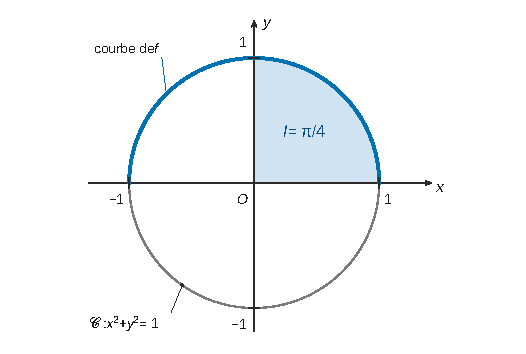
\includegraphics{figures/p1-q3b-quart-de-disque.pdf}
\caption*{Figure 1 --- La courbe de f est le demi-cercle supérieur de 𝒞 ; I est
l'aire du quart de disque, soit π/4}
\end{figure}

\hypertarget{partie-b-duxe9nombrement-de-points-dans-un-disque}{%
\subsection{Partie B : Dénombrement de points dans un disque}\label{partie-b-duxe9nombrement-de-points-dans-un-disque}}

\(D_n=\{(x,y)\in\mathbb Z^2,\ x^2+y^2\leqslant n^2\}\), \(Q_n=\{(x,y)\in(\mathbb N^*)^2,\ x^2+y^2\leqslant n^2\}\).

\hypertarget{section}{%
\subsubsection{4.}\label{section}}

\begin{itemize}
\tightlist
\item
  \(D_1\) : on a \(x^2\leqslant1\) et \(y^2\leqslant 1\), donc \(x,y\in\{-1,0,1\}\).

  \begin{itemize}
  \tightlist
  \item
    Parmi ces 9 couples, les couples \((\pm1,\pm1)\) donnent \(2>1\).
  \item
    Il reste \((0,0),(\pm1,0),(0,\pm1)\).
  \end{itemize}
\item
  \(Q_1\) : si \(x,y\geqslant1\), alors \(x^2+y^2\geqslant2>1\), donc \(Q_1=\varnothing\).
\item
  \(Q_3\) : \(y\geqslant1\) impose \(x^2\leqslant 8\), donc \(x\in\{1,2\}\).

  \begin{itemize}
  \tightlist
  \item
    Pour \(x=1\) : \(y^2\leqslant8\), donc \(y\in\{1,2\}\).
  \item
    Pour \(x=2\) : \(y^2\leqslant5\), donc \(y\in\{1,2\}\).
  \item
    Donc \(Q_3=\{(1,1),(1,2),(2,1),(2,2)\}\).
  \end{itemize}
\end{itemize}

\equationajustee{\boxed{\begin{aligned}
\operatorname{Card}(D_1)&=5\\
\operatorname{Card}(Q_1)&=0\\
\operatorname{Card}(Q_3)&=4
\end{aligned}}}

\hypertarget{a-3}{%
\subsubsection{5. (a)}\label{a-3}}

On partitionne \(D_n\) en trois parties disjointes :

\begin{itemize}
\tightlist
\item
  l'origine \((0,0)\) : 1 point ;
\item
  les points non nuls situés sur un axe, au nombre de \(4n\) :

  \begin{itemize}
  \tightlist
  \item
    \((x,0)\) avec \(x\neq0\) est dans \(D_n\) si et seulement si \(|x|\leqslant n\), soit \(2n\) points ;
  \item
    de même, il y a \(2n\) points \((0,y)\) ;
  \end{itemize}
\item
  les points \((x,y)\) de \(D_n\) tels que \(x\neq0\) et \(y\neq0\) :

  \begin{itemize}
  \tightlist
  \item
    l'application \((x,y)\mapsto(|x|,|y|)\) envoie cet ensemble dans \(Q_n\), car \(|x|,|y|\in\mathbb N^*\) et \(|x|^2+|y|^2=x^2+y^2\) ;
  \item
    tout \((a,b)\in Q_n\) a exactement quatre antécédents distincts \((\pm a,\pm b)\), tous dans \(D_n\) (symétries par rapport aux axes et à l'origine) ;
  \item
    cet ensemble a donc \(4\operatorname{Card}(Q_n)\) éléments.
  \end{itemize}
\end{itemize}

\equationajustee{\boxed{\forall n\in\mathbb N^*,\quad \operatorname{Card}(D_n)=1+4n+4\operatorname{Card}(Q_n).}}

\begin{figure}[H]
\centering
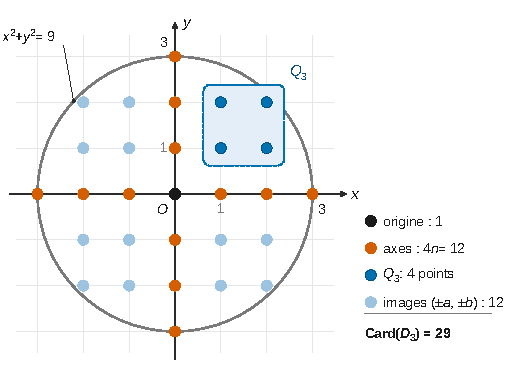
\includegraphics{figures/p1-q5a-points-d3.pdf}
\caption*{Figure 2 --- Les 29 points de D₃ : l'origine, 4n = 12 points sur les
axes et les quatre copies (±a, ±b) des 4 points de Q₃}
\end{figure}

\hypertarget{b-3}{%
\subsubsection{5. (b)}\label{b-3}}

Si \((x,y)\in Q_n\), alors \(y\geqslant1\), donc \(x^2\leqslant n^2-1<n^2\) et \(x\in\llbracket1,n-1\rrbracket\).

On compte \(Q_n\) par colonnes : pour \(x\in\llbracket1,n-1\rrbracket\) fixé et \(y\in\mathbb N^*\),

\equationajustee{\begin{aligned}
(x,y)\in Q_n&\iff y^2\leqslant n^2-x^2\\
&\iff y\leqslant\sqrt{n^2-x^2}\\
&\iff y\leqslant\big\lfloor\sqrt{n^2-x^2}\big\rfloor.
\end{aligned}}

La deuxième équivalence vient de la croissance de la racine sur \(\mathbb R_+\) (\(y>0\)). La troisième vient de ce que \(y\) est entier.

En effet, si \(y\leqslant t\) avec \(y\in\mathbb Z\), alors \(y\leqslant\lfloor t\rfloor\) par définition de la partie entière (plus grand entier inférieur ou égal à \(t\)). La réciproque vient de \(\lfloor t\rfloor\leqslant t\).

La colonne d'abscisse \(x\) contient donc \(\lfloor\sqrt{n^2-x^2}\rfloor\) points. D'où, pour tout \(n\in\mathbb N^*\) :

\equationajustee{\boxed{\operatorname{Card}(Q_n)=\sum_{x=1}^{n-1}\big\lfloor\sqrt{n^2-x^2}\big\rfloor}}

(somme vide, nulle, pour \(n=1\), en accord avec \(Q_1=\varnothing\)).

\hypertarget{c-1}{%
\subsubsection{5. (c)}\label{c-1}}

Pour tout réel \(t\), \(t-1<\lfloor t\rfloor\leqslant t\). On l'applique à \(t=\sqrt{n^2-x^2}\) et on somme pour \(x\in\llbracket1,n-1\rrbracket\) (\(n-1\) termes) :

\equationajustee{\sum_{x=1}^{n-1}\sqrt{n^2-x^2}-(n-1)\leqslant\operatorname{Card}(Q_n)\leqslant\sum_{x=1}^{n-1}\sqrt{n^2-x^2}.}

Le terme \(x=n\) de \(\sum_{x=1}^{n}\sqrt{n^2-x^2}\) est nul, donc \(\sum_{x=1}^{n-1}\sqrt{n^2-x^2}=\sum_{x=1}^{n}\sqrt{n^2-x^2}\).

Ainsi, pour tout \(n\in\mathbb N^*\) :

\equationajustee{\boxed{1-n+\sum_{x=1}^{n}\sqrt{n^2-x^2}\leqslant\operatorname{Card}(Q_n)\leqslant\sum_{x=1}^{n}\sqrt{n^2-x^2}.}}

\hypertarget{a-4}{%
\subsubsection{6. (a)}\label{a-4}}

Pour \(x\in\llbracket1,n\rrbracket\), \(\sqrt{n^2-x^2}=n\sqrt{1-(x/n)^2}\) (\(n>0\)), donc

\equationajustee{\begin{aligned}
R_n&=\frac1{n^2}\sum_{x=1}^n n\sqrt{1-\Big(\frac xn\Big)^2}\\
&=\frac1n\sum_{x=1}^{n}f\Big(\frac xn\Big),
\end{aligned}}

avec \(f(u)=\sqrt{1-u^2}\).

\textbf{\(R_n\) est la somme de Riemann (à droite, pas \(1/n\)) de la fonction \(f:u\mapsto\sqrt{1-u^2}\) sur le segment \([0,1]\).} Elle est associée à la subdivision régulière \(\big(\frac kn\big)_{0\leqslant k\leqslant n}\).

\begin{figure}[H]
\centering
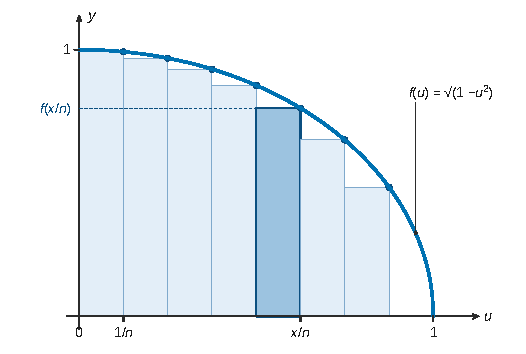
\includegraphics{figures/p1-q6a-somme-riemann.pdf}
\caption*{Figure 3 --- Somme de Riemann Rₙ pour n = 8 : rectangles de largeur 1/n
et de hauteur f(x/n), prise à droite, sous la courbe de f}
\end{figure}

\hypertarget{b-4}{%
\subsubsection{6. (b)}\label{b-4}}

\(f\) est continue sur le segment \([0,1]\), donc la suite de ses sommes de Riemann converge vers son intégrale :

\equationajustee{\boxed{R_n\xrightarrow[n\to+\infty]{}\int_0^1\sqrt{1-u^2}\,\mathrm du=I=\frac\pi4.}}

\hypertarget{c-2}{%
\subsubsection{6. (c)}\label{c-2}}

En divisant l'encadrement de 5(c) par \(n^2>0\) :

\equationajustee{\frac{1-n}{n^2}+R_n\leqslant\frac{\operatorname{Card}(Q_n)}{n^2}\leqslant R_n .}

Comme \(\frac{1-n}{n^2}\to0\) et \(R_n\to\frac\pi4\), le théorème des gendarmes donne \(\frac{\operatorname{Card}(Q_n)}{n^2}\to\frac\pi4\neq0\), c'est-à-dire

\equationajustee{\boxed{\operatorname{Card}(Q_n)\underset{n\to+\infty}{\sim}\frac{\pi n^2}{4}.}}

Avec 5(a) :

\equationajustee{\begin{aligned}
\frac{\operatorname{Card}(D_n)}{n^2}&=\frac1{n^2}+\frac4n+4\,\frac{\operatorname{Card}(Q_n)}{n^2}\\
&\longrightarrow 0+0+4\cdot\frac\pi4=\pi.
\end{aligned}}

Cette limite est non nulle, donc

\equationajustee{\boxed{\operatorname{Card}(D_n)\underset{n\to+\infty}{\sim}\pi n^2.}}

\hypertarget{partie-c-convergence-en-loi}{%
\subsection{Partie C : Convergence en loi}\label{partie-c-convergence-en-loi}}

\(X_n,Y_n\hookrightarrow\mathcal U(\llbracket-n,n\rrbracket)\), et \((X_1,\dots,X_N,Y_1,\dots,Y_N)\) sont mutuellement indépendantes pour tout \(N\).

On a \(Z_n=1\) si \(X_n^2+Y_n^2\leqslant n^2\), et \(0\) sinon.

\hypertarget{a-5}{%
\subsubsection{7. (a)}\label{a-5}}

\(X_n\) est finie, de loi \(P(X_n=k)=\frac1{2n+1}\) pour \(k\in\llbracket-n,n\rrbracket\), donc

\equationajustee{\begin{aligned}
E(X_n)&=\frac{1}{2n+1}\sum_{k=-n}^{n}k\\
&=0,
\end{aligned}}

la somme étant nulle (les termes \(k\) et \(-k\) se compensent ; le changement d'indice \(k\mapsto-k\) montre qu'elle est égale à son opposée).

\equationajustee{\boxed{\forall n\in\mathbb N^*,\quad E(X_n)=0.}}

\hypertarget{b-5}{%
\subsubsection{7. (b)}\label{b-5}}

Par la formule de König-Huygens et 7(a), \(V(X_n)=E(X_n^2)-E(X_n)^2=E(X_n^2)\). Par le théorème de transfert :

\equationajustee{\begin{aligned}
E(X_n^2)&=\frac1{2n+1}\sum_{k=-n}^nk^2\\
&=\frac{2}{2n+1}\sum_{k=1}^nk^2\\
&=\frac{2}{2n+1}\cdot\frac{n(n+1)(2n+1)}{6}\\
&=\frac{n(n+1)}3 .
\end{aligned}}

\equationajustee{\boxed{\forall n\in\mathbb N^*,\quad V(X_n)=\frac{n(n+1)}{3}.}}

\hypertarget{a-6}{%
\subsubsection{8. (a)}\label{a-6}}

Soit \(N\in\mathbb N^*\). Pour tout \(n\), \(Z_n=h_n(X_n,Y_n)\) avec

\equationajustee{h_n(x,y)=\begin{cases}1&\text{si } x^2+y^2\leqslant n^2,\\0&\text{sinon.}\end{cases}}

La famille \((X_1,\dots,X_N,Y_1,\dots,Y_N)\) est mutuellement indépendante et les paquets \(\{X_1,Y_1\},\dots,\{X_N,Y_N\}\) sont disjoints.

D'après le lemme des coalitions, \(h_1(X_1,Y_1),\dots,h_N(X_N,Y_N)\), c'est-à-dire \(Z_1,\dots,Z_N\), sont mutuellement indépendantes. Ceci valant pour tout \(N\) :

\textbf{les variables aléatoires \((Z_n)_{n\in\mathbb N^*}\) sont mutuellement indépendantes.}

\hypertarget{b-6}{%
\subsubsection{8. (b)}\label{b-6}}

\(Z_n(\Omega)\subset\{0,1\}\), donc \(Z_n\) suit une loi de Bernoulli de paramètre \(p_n=P(Z_n=1)\).

Les variables \(X_n\) et \(Y_n\) sont indépendantes. Pour \((x,y)\in\llbracket-n,n\rrbracket^2\), on a donc \(P(X_n=x,Y_n=y)=\frac{1}{(2n+1)^2}\).

Le couple est ainsi uniforme sur \(\llbracket-n,n\rrbracket^2\), de cardinal \((2n+1)^2\).

Si \((x,y)\in\mathbb Z^2\) vérifie \(x^2+y^2\leqslant n^2\), alors \(|x|\leqslant n\) et \(|y|\leqslant n\).

L'ensemble des couples favorables de \(\llbracket-n,n\rrbracket^2\) est donc exactement \(D_n\). Donc

\equationajustee{\boxed{Z_n\hookrightarrow\mathcal B\left(\frac{\operatorname{Card}(D_n)}{(2n+1)^2}\right).}}

\hypertarget{a-7}{%
\subsubsection{9. (a)}\label{a-7}}

Soient \((T_n)\) une suite de variables aléatoires et \(T\) une variable aléatoire, toutes à valeurs dans \(\mathbb N\).

La suite \((T_n)\) converge en loi vers \(T\) si et seulement si, pour tout \(k\in\mathbb N\) :

\equationajustee{\boxed{P(T_n=k)\xrightarrow[n\to+\infty]{}P(T=k).}}

\hypertarget{b-7}{%
\subsubsection{9. (b)}\label{b-7}}

D'après 6(c), \(\operatorname{Card}(D_n)\sim\pi n^2\), et \((2n+1)^2\sim4n^2\).

Par quotient d'équivalents, \(p_n\sim\frac{\pi n^2}{4n^2}=\frac\pi4\), donc \(p_n\to\frac\pi4\).

Les \(Z_n\) sont à valeurs dans \(\{0,1\}\subset\mathbb N\) et

\equationajustee{\begin{aligned}
P(Z_n=1)&=p_n\to\frac\pi4,\\
P(Z_n=0)&=1-p_n\to1-\frac\pi4,\\
P(Z_n=k)&=0\ \text{ pour } k\geqslant2.
\end{aligned}}

Comme \(3<\pi<4\), on a \(\frac\pi4\in\,]0,1[\) et l'on peut considérer \(Z\hookrightarrow\mathcal B(\pi/4)\).

Les limites ci-dessus sont exactement les \(P(Z=k)\), \(k\in\mathbb N\). Donc \((Z_n)\) converge en loi vers \(Z\), avec

\equationajustee{\boxed{\begin{aligned}
Z&\hookrightarrow\mathcal B\Big(\frac\pi4\Big)\\
E(Z)&=\frac\pi4\\
V(Z)&=\frac\pi4\Big(1-\frac\pi4\Big)
\end{aligned}}}

\hypertarget{a-8}{%
\subsubsection{10. (a)}\label{a-8}}

Notons \(\overline Z_n=\frac1n\sum_{k=1}^nZ_k\) la moyenne empirique. Par linéarité de l'espérance et 8(b), \(E(\overline Z_n)=\frac1n\sum_{k=1}^n p_k\).

La suite \((p_k)\) converge vers \(\frac\pi4\) (question 9(b)), donc par le théorème de Cesàro :

\equationajustee{\boxed{E(\overline Z_n)=\frac1n\sum_{k=1}^np_k\xrightarrow[n\to+\infty]{}\frac\pi4.}}

\hypertarget{b-8}{%
\subsubsection{10. (b)}\label{b-8}}

Les \(Z_k\) sont mutuellement indépendantes (8(a)), donc la variance de leur somme est la somme des variances :

\equationajustee{\begin{aligned}
V(\overline Z_n)&=\frac1{n^2}\sum_{k=1}^nV(Z_k)\\
&=\frac1n\cdot\Big(\frac1n\sum_{k=1}^np_k(1-p_k)\Big).
\end{aligned}}

Par continuité de \(t\mapsto t(1-t)\), \(p_k(1-p_k)\to\frac\pi4\big(1-\frac\pi4\big)\). Par Cesàro, la parenthèse converge donc vers ce réel ; multipliée par \(\frac1n\to0\), elle donne

\equationajustee{\boxed{V(\overline Z_n)\xrightarrow[n\to+\infty]{}0.}}

\hypertarget{probluxe8me-2}{%
\section{Problème 2}\label{probluxe8me-2}}

\hypertarget{partie-a-matrice-de-carruxe9-nul}{%
\subsection{Partie A : Matrice de carré nul}\label{partie-a-matrice-de-carruxe9-nul}}

\hypertarget{a-9}{%
\subsubsection{1. (a)}\label{a-9}}

\equationajustee{\begin{aligned}
S^2&=O_2,\\
T^2&=\begin{pmatrix}0&0&0\\0&0&0\\2&0&0\end{pmatrix}\neq O_3,\\
U^2&=O_3.
\end{aligned}}

\textbf{Les matrices de carré nul sont \(S\) et \(U\)} ; \(T\) ne l'est pas.

\hypertarget{b-9}{%
\subsubsection{1. (b)}\label{b-9}}

Soit \(A\) telle que \(A^2=O_n\). Soit \(\lambda\) une valeur propre de \(A\), de vecteur propre \(X\neq0\) : \(AX=\lambda X\). Alors

\equationajustee{\begin{aligned}
A^2X&=A(\lambda X)\\
&=\lambda AX\\
&=\lambda^2X.
\end{aligned}}

Or \(A^2X=0\). Donc \(\lambda^2X=0\) avec \(X\neq0\), d'où \(\lambda^2=0\) :

\equationajustee{\boxed{\lambda=0.}}

\hypertarget{c-3}{%
\subsubsection{1. (c)}\label{c-3}}

Soit \(A=(a_{ij})\) symétrique avec \(A^2=O_n\). Le coefficient diagonal \((i,i)\) de \(A^2\) vaut

\equationajustee{\begin{aligned}
(A^2)_{ii}&=\sum_{k=1}^na_{ik}a_{ki}\\
&=\sum_{k=1}^na_{ik}^2
\end{aligned}}

car \(a_{ki}=a_{ik}\). Il est nul : une somme de carrés de réels nulle a tous ses termes nuls, donc \(a_{ik}=0\) pour tous \(i,k\) :

\equationajustee{\boxed{A=O_n.}}

(Variante : \(A\) symétrique réelle est diagonalisable, \(A=PDP^{-1}\) avec \(D\) diagonale formée des valeurs propres. Celles-ci sont toutes nulles d'après 1(b), donc \(D=O_n\) et \(A=O_n\).)

\hypertarget{a-10}{%
\subsubsection{2. (a)}\label{a-10}}

Si \(m=1\), \(A=O_2\) donc \(A^2=O_2\) ; si \(m=2\), \(A^2=O_2\) est l'hypothèse. \textbf{Dans les deux cas \(A^2=O_2\).}

\hypertarget{b-10}{%
\subsubsection{2. (b)}\label{b-10}}

Supposons que l'on ait \(A^2X=0\) pour tout \(X\in\mathcal M_{2,1}(\mathbb R)\). Prenons \(X=E_1\) puis \(X=E_2\) (colonnes de la base canonique).

Les deux colonnes de \(A^2\) sont alors nulles et \(A^2=O_2\), ce qui est exclu.

\textbf{Il existe donc \(X\in\mathcal M_{2,1}(\mathbb R)\) tel que \(A^2X\neq0\).}

\hypertarget{c-4}{%
\subsubsection{2. (c)}\label{c-4}}

On a \(A^3=O_2\), donc \(A^4=A\cdot A^3=O_2\). Soient \(\alpha,\beta,\gamma\) réels tels que \(\alpha X+\beta AX+\gamma A^2X=0\).

\begin{itemize}
\tightlist
\item
  En multipliant à gauche par \(A^2\) : \(\alpha A^2X+\beta A^3X+\gamma A^4X=\alpha A^2X=0\). Comme \(A^2X\neq0\), \(\alpha=0\).
\item
  Il reste \(\beta AX+\gamma A^2X=0\) ; en multipliant par \(A\) : \(\beta A^2X=0\), donc \(\beta=0\).
\item
  Il reste \(\gamma A^2X=0\), donc \(\gamma=0\).
\end{itemize}

La famille \((X,AX,A^2X)\) est libre. Or \(\mathcal M_{2,1}(\mathbb R)\) est de dimension \(2\), et une famille libre y compte au plus \(2\) vecteurs : contradiction.

Donc \(A^2=O_2\), et avec 2(a) :

\textbf{pour \(A\in\mathcal M_2(\mathbb R)\), s'il existe \(m\in\{1,2,3\}\) tel que \(A^m=O_2\), alors \(A^2=O_2\).}

\hypertarget{section-1}{%
\subsubsection{3.}\label{section-1}}

Soient \(M,N\in\mathcal M_2(\mathbb R)\) avec \((MN)^2=O_2\). Par associativité,

\equationajustee{\begin{aligned}
(NM)^3&=NMNMNM\\
&=N(MN)(MN)M\\
&=N(MN)^2M\\
&=O_2 .
\end{aligned}}

La matrice \(NM\in\mathcal M_2(\mathbb R)\) vérifie \((NM)^3=O_2\). D'après la question 2 (avec \(m=3\)), \textbf{\((NM)^2=O_2\) : \(NM\) est de carré nul.}

\hypertarget{partie-b-endomorphisme-de-mathbb-r3-de-carruxe9-nul}{%
\subsection{\texorpdfstring{Partie B : Endomorphisme de \(\mathbb R^3\) de carré nul}{Partie B : Endomorphisme de \textbackslash mathbb R\^{}3 de carré nul}}\label{partie-b-endomorphisme-de-mathbb-r3-de-carruxe9-nul}}

\hypertarget{section-2}{%
\subsubsection{4.}\label{section-2}}

Si \(u=0\), prenons une base \(\mathcal B\) quelconque de \(\mathbb R^3\) (par exemple la base canonique).

Toutes les colonnes de \(\operatorname{Mat}_{\mathcal B}(u)\) sont nulles : \(\operatorname{Mat}_{\mathcal B}(u)=O_3\).

C'est la forme voulue avec \textbf{\(\varepsilon=0\) (et n'importe quelle base \(\mathcal B\)).}

\hypertarget{a-11}{%
\subsubsection{5. (a)}\label{a-11}}

Comme \(u\neq0\), il existe \(a\in\mathbb R^3\) tel que \(u(a)\neq0\).

Soient \(\alpha,\beta\) réels tels que \(\alpha u(a)+\beta a=0\). En appliquant \(u\) (linéaire) :

\equationajustee{\alpha u^2(a)+\beta u(a)=\beta u(a)=0.}

Donc \(\beta=0\) puisque \(u(a)\neq0\) ; puis \(\alpha u(a)=0\) donne \(\alpha=0\).

\textbf{La famille \((u(a),a)\) est libre.}

\hypertarget{b-11}{%
\subsubsection{5. (b)}\label{b-11}}

\((u(a),a)\) est une famille libre de \(\mathbb R^3\), espace de dimension finie \(3\).

D'après le théorème de la base incomplète, on peut la compléter en une base de \(\mathbb R^3\). Comme elle a \(2\) vecteurs, il suffit d'en ajouter un.

\textbf{Il existe \(e\in\mathbb R^3\) tel que \(\mathcal A=(u(a),a,e)\) soit une base de \(\mathbb R^3\).}

\hypertarget{c-5}{%
\subsubsection{5. (c)}\label{c-5}}

On a, dans la base \(\mathcal A\) :

\equationajustee{\begin{aligned}
a&=0\cdot u(a)+1\cdot a+0\cdot e,\\
u(a)&=1\cdot u(a)+0\cdot a+0\cdot e.
\end{aligned}}

Par unicité des coordonnées dans la base \(\mathcal A\) :

\equationajustee{\boxed{\begin{aligned}
a_1&=0\\
u(a)_1&=1
\end{aligned}}}

\hypertarget{a-12}{%
\subsubsection{6. (a)}\label{a-12}}

D'après 5(c), et puisque \(u(u(a))=u^2(a)=0\) a une première coordonnée nulle :

\equationajustee{\begin{aligned}
\varphi(a)&=(a_1,u(a)_1)=(0,1),\\
\varphi(u(a))&=(u(a)_1,u^2(a)_1)=(1,0).
\end{aligned}}

L'image de \(\varphi\) contient la base \(\big((1,0),(0,1)\big)\) de \(\mathbb R^2\).

Donc \(\operatorname{Im}\varphi=\mathbb R^2\) et

\equationajustee{\boxed{\operatorname{rg}(\varphi)=2.}}

Par le théorème du rang appliqué à \(\varphi\in\mathcal L(\mathbb R^3,\mathbb R^2)\) : \(\dim\operatorname{Ker}\varphi=3-2=1\).

\textbf{\(\operatorname{Ker}(\varphi)\) est une droite vectorielle de \(\mathbb R^3\).}

\hypertarget{b-12}{%
\subsubsection{6. (b)}\label{b-12}}

Soit \(e'\) un vecteur directeur de \(\operatorname{Ker}\varphi\) : \(e'\neq0\) et \(\varphi(e')=(0,0)\).

Soient \(\alpha,\beta,\gamma\) réels tels que \(\alpha u(a)+\beta e'+\gamma a=0\). En appliquant \(\varphi\) (linéaire) :

\equationajustee{\alpha(1,0)+\beta(0,0)+\gamma(0,1)=(\alpha,\gamma)=(0,0),}

donc \(\alpha=\gamma=0\), puis \(\beta e'=0\) et \(\beta=0\).

La famille \(\mathcal B=(u(a),e',a)\) est libre et a \(3=\dim\mathbb R^3\) vecteurs : \textbf{\(\mathcal B\) est une base de \(\mathbb R^3\).}

\hypertarget{c-6}{%
\subsubsection{6. (c)}\label{c-6}}

Comme \(\varphi(e')=(e'_1,u(e')_1)=(0,0)\), on a \(u(e')_1=0\). Alors

\equationajustee{\varphi(u(e'))=\big(u(e')_1,\ u^2(e')_1\big)=(0,0)}

car \(u^2=0\). Donc \textbf{\(u(e')\in\operatorname{Ker}\varphi\)}.

Ce noyau est la droite \(\operatorname{Vect}(e')\) : il existe \(\mu\in\mathbb R\) tel que \(u(e')=\mu e'\).

Ainsi \(e'\neq0\) est un vecteur propre de \(u\) associé à \(\mu\). Comme en 1(b), on applique \(u\) :

\equationajustee{\begin{aligned}
0&=u^2(e')\\
&=\mu\,u(e')\\
&=\mu^2e'.
\end{aligned}}

D'où \(\mu^2=0\) puisque \(e'\neq0\). Ainsi \(\mu=0\) et

\equationajustee{\boxed{u(e')=0.}}

\hypertarget{d}{%
\subsubsection{6. (d)}\label{d}}

Dans la base \(\mathcal B=(u(a),e',a)\) :

\equationajustee{\begin{aligned}
u(u(a))&=0,\\
u(e')&=0\quad\text{(question 6(c))},\\
u(a)&=1\cdot u(a)+0\cdot e'+0\cdot a.
\end{aligned}}

Donc

\equationajustee{\operatorname{Mat}_{\mathcal B}(u)=\begin{pmatrix}0&0&1\\0&0&0\\0&0&0\end{pmatrix},}

forme voulue avec \(\varepsilon=1\). On conclut avec la question 4 (cas \(u=0\), \(\varepsilon=0\)).

\textbf{Pour tout endomorphisme \(u\) de \(\mathbb R^3\) de carré nul, il existe une base \(\mathcal B\) de \(\mathbb R^3\) et \(\varepsilon\in\{0,1\}\) tels que}

\equationajustee{\boxed{\operatorname{Mat}_{\mathcal B}(u)=\begin{pmatrix}0&0&\varepsilon\\0&0&0\\0&0&0\end{pmatrix},}}

\textbf{avec \(\varepsilon=0\) si \(u=0\) et \(\varepsilon=1\) sinon.}

\begin{figure}[H]
\centering
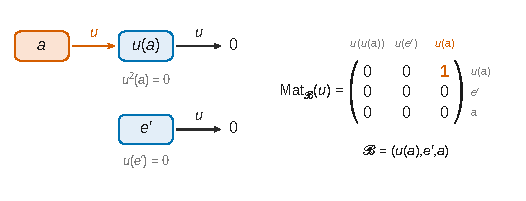
\includegraphics{figures/p2-q6-chaine-base.pdf}
\caption*{Figure 4 --- Action de u sur la base 𝓑 = (u(a), e′, a) : a ↦ u(a) ↦ 0 et
e′ ↦ 0, d'où la matrice de u dans 𝓑}
\end{figure}

\hypertarget{partie-c-avec-un-duxe9}{%
\subsection{Partie C : Avec un dé}\label{partie-c-avec-un-duxe9}}

Les lancers sont indépendants et chacun donne \(6\) avec probabilité \(\frac16\). L'événement « on n'obtient jamais six fois le \(6\) » est de probabilité nulle et n'affecte aucun calcul.

\hypertarget{a-13}{%
\subsubsection{7. (a)}\label{a-13}}

\begin{figure}[H]
\centering
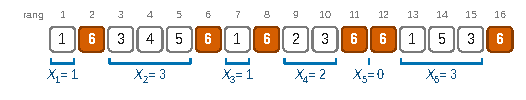
\includegraphics{figures/p2-partie-c-frise-lancers.pdf}
\caption*{Figure 5 --- Exemple de l'énoncé : les six découpent la suite des
lancers ; X₅ = 0 pour deux six consécutifs}
\end{figure}

Soit \(G\) le rang du premier six. C'est le temps d'attente du premier succès dans une suite d'épreuves de Bernoulli indépendantes de paramètre \(\frac16\).

Ainsi \(G\hookrightarrow\mathcal G(\frac16)\), \(G(\Omega)=\mathbb N^*\), et pour \(k\in\mathbb N^*\) :

\equationajustee{P(G=k)=\frac16\Big(\frac56\Big)^{k-1}.}

Le nombre de lancers avant le premier six est \(X_1=G-1\), donc \(X_1(\Omega)=\mathbb N\) et, pour tout \(n\in\mathbb N\) :

\equationajustee{\boxed{\begin{aligned}
P(X_1=n)&=P(G=n+1)\\
&=\frac16\Big(\frac56\Big)^{n}.
\end{aligned}}}

Avec \(p=\frac16\) :

\equationajustee{\begin{aligned}
E(G)&=\frac1p=6,\\
V(G)&=\frac{1-p}{p^2}\\
&=\frac{5/6}{1/36}=30.
\end{aligned}}

Donc :

\equationajustee{\boxed{\begin{aligned}
E(X_1)&=E(G)-1=5\\
V(X_1)&=V(G)=30
\end{aligned}}}

\hypertarget{b-13}{%
\subsubsection{7. (b)}\label{b-13}}

Soient \(n_1,\dots,n_6\in\mathbb N\), et notons \(H\) l'événement \(\{X_1=n_1,\dots,X_6=n_6\}\).

Il signifie exactement que, parmi les \(n_1+\dots+n_6+6\) premiers lancers, ceux de rangs

\equationajustee{n_1+1,\quad n_1+n_2+2,\quad\dots,\quad n_1+\dots+n_6+6}

donnent \(6\), et que tous les autres donnent autre chose que \(6\). Par indépendance des lancers :

\equationajustee{P(H)=\prod_{i=1}^6\frac16\Big(\frac56\Big)^{n_i}.}

En sommant sur les \(n_j\), \(j\neq i\) (séries géométriques de somme \(1\)), on obtient

\equationajustee{P(X_i=n_i)=\frac16\Big(\frac56\Big)^{n_i},}

et la loi conjointe est le produit des lois marginales.

\textbf{Les variables \(X_1,\dots,X_6\) sont mutuellement indépendantes et suivent toutes la même loi que \(X_1\)} (géométrique décalée : \(X_i+1\hookrightarrow\mathcal G(\frac16)\)), d'espérance \(5\) et de variance \(30\).

\hypertarget{a-14}{%
\subsubsection{8. (a)}\label{a-14}}

\(P(X_i=0)=\frac16\) pour tout \(i\). Par indépendance mutuelle de \(X_1,X_4,X_6\) :

\equationajustee{\boxed{\begin{aligned}
P(X_1=X_4=X_6=0)&=\Big(\frac16\Big)^3\\
&=\frac1{216}.
\end{aligned}}}

\hypertarget{b-14}{%
\subsubsection{8. (b)}\label{b-14}}

Par la formule de Poincaré et l'indépendance de \(X_2\) et \(X_5\) :

\equationajustee{\begin{aligned}
P(\{X_2=0\}\cup\{X_5=0\})&=\frac16+\frac16-\frac16\cdot\frac16\\
&=\boxed{\frac{11}{36}.}
\end{aligned}}

(Contrôle par le complémentaire : \(1-\big(\frac56\big)^2=\frac{11}{36}\).)

\hypertarget{section-3}{%
\subsubsection{9.}\label{section-3}}

Écrivons \(A=A(\omega)\). Un calcul direct donne

\equationajustee{A^2=\begin{pmatrix}X_1^2&X_1X_2+X_2X_4&X_1X_3+X_2X_5+X_3X_6\\0&X_4^2&X_4X_5+X_5X_6\\0&0&X_6^2\end{pmatrix}.}

Si \(A^2=O_3\), les coefficients diagonaux donnent \(X_1=X_4=X_6=0\).

Alors \(A^2\) se réduit à la matrice dont le seul coefficient éventuellement non nul est \((A^2)_{13}=X_2X_5\).

Réciproquement, si \(X_1=X_4=X_6=0\) et \(X_2X_5=0\), tous les coefficients de \(A^2\) sont nuls. Donc

\equationajustee{\begin{aligned}
\{A^2=O_3\}&=\big(\{X_1=0\}\cap\{X_4=0\}\cap\{X_6=0\}\big)\\
&\quad\cap\big(\{X_2=0\}\cup\{X_5=0\}\big).
\end{aligned}}

Le premier événement ne dépend que de \((X_1,X_4,X_6)\), le second que de \((X_2,X_5)\).

Ces paquets sont disjoints et \(X_1,\dots,X_6\) sont mutuellement indépendantes (7(b)). Par le lemme des coalitions, les deux événements sont donc indépendants. Avec 8(a) et 8(b) :

\equationajustee{\boxed{\begin{aligned}
P(A^2=O_3)&=\frac1{216}\cdot\frac{11}{36}\\
&=\frac{11}{7776}\\
&\approx1{,}41\times10^{-3}.
\end{aligned}}}

\end{document}
